\documentclass[]{report}
\usepackage{nips13submit_e,times}
\usepackage[utf8x]{inputenc}
\usepackage{amsfonts}
\usepackage{indentfirst}
\usepackage{hyperref}
\usepackage{graphicx}
\usepackage{enumerate}
\usepackage{amsmath}
\usepackage{subfigure}
\usepackage{amsopn}
\title{Project-II by group TORONTO}
\author{Michalina Pacholska \And Jakub Sygnowski}
\nipsfinalcopy
\newcommand{\mychapter}[2]{
    \setcounter{chapter}{#1}
    \setcounter{section}{0}
    \chapter*{#2}
}


\begin{document}
\begingroup
\renewcommand{\cleardoublepage}{}
\renewcommand{\clearpage}{}
\mychapter{1}{Person detection}
\endgroup

\section{Problem and dataset descriptions}
  During the project, we were first given a set of images and labels indicating whether there is a person on the image. We also were given features (HOG, \cite{hog}) extracted from the images and we were supposed to analyze them and train our algorithms only on those extracted features (not on images). Then, a week before the deadline, we were given a test set of features for which we should give our predictions. 

  Train dataset contains $8545$ images and labels ($1$ - person, $0$ - not), and for every image $9360$ features in a form of a $26\times10\times36$ cube. There are $1237$ images with a person.

\begin{figure}[!h]
  \center
  \subfigure[picture]{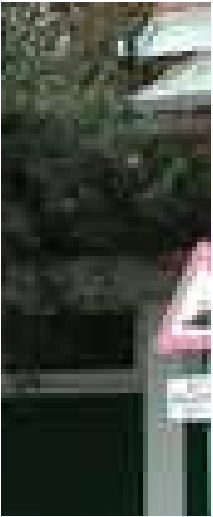
\includegraphics[height=1.7in]{../figures/examplePicture-crop.pdf} \label{fig:examplePicture}}
  \;
  \subfigure[features]{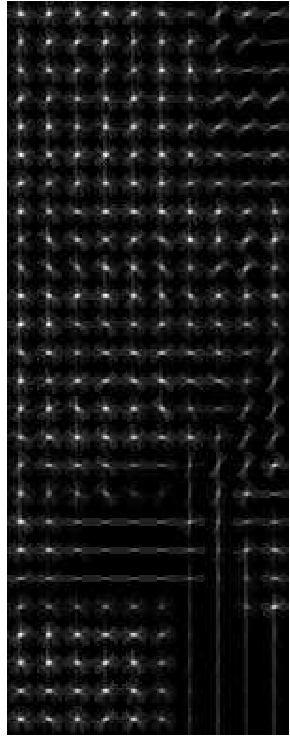
\includegraphics[height=1.7in]{../figures/exampleFeature-crop.pdf} \label{fig:exampleFeature}}
  \caption{ \ref{fig:examplePicture} picture No 200 and \ref{fig:exampleFeature} features extracted form it, using Piotr's toolbox \cite{piotr}
  }
\end{figure}

\section{Data analysis and preparation}
  First two dimensions $26\times10$ of features for particular image correspond to the position of subimage from which those features were extracted. The third dimension corresponds to the directions of "edges" on that part of image. White color and big number indicates that there is an edge (see \ref{fig:examplePicture} and \ref{fig:exampleFeature}). Values of features are between $0$ and $0.2$ and normalization doesn't change much their distribution.
  \begin{figure}[!h]
  \center
  \subfigure[original data]{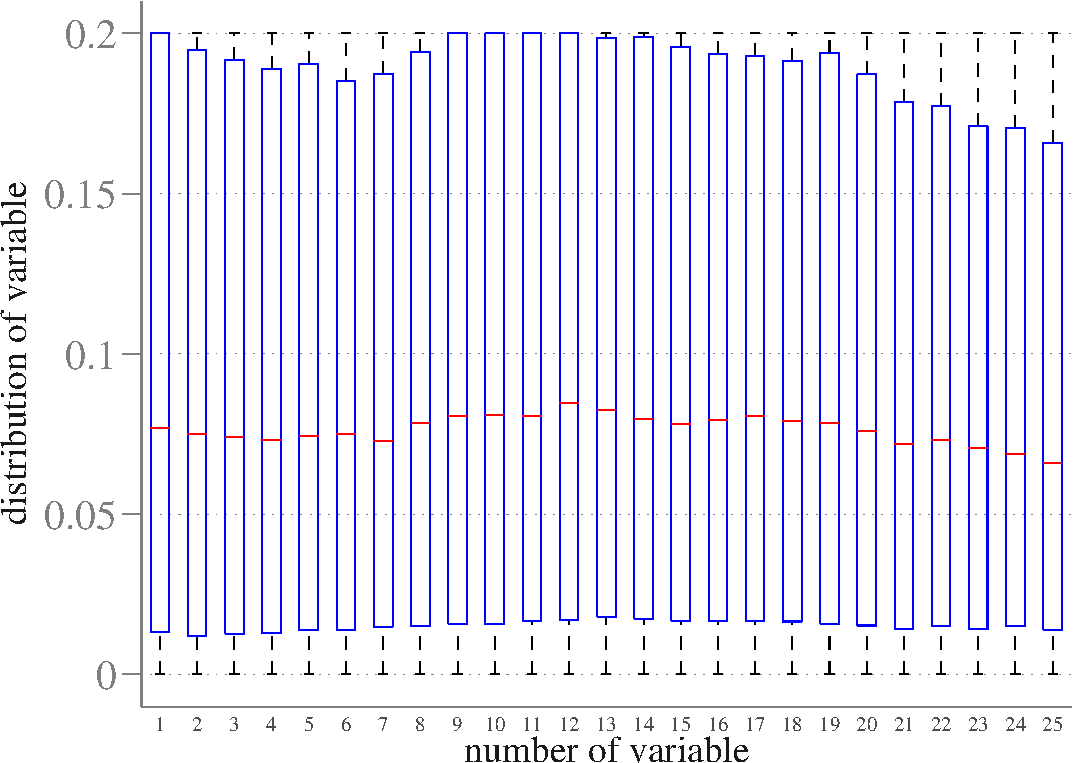
\includegraphics[height=1.8in]{../figures/boxplot1-crop.pdf} \label{fig:boxplot1}}
  \;
  \subfigure[after normalization]{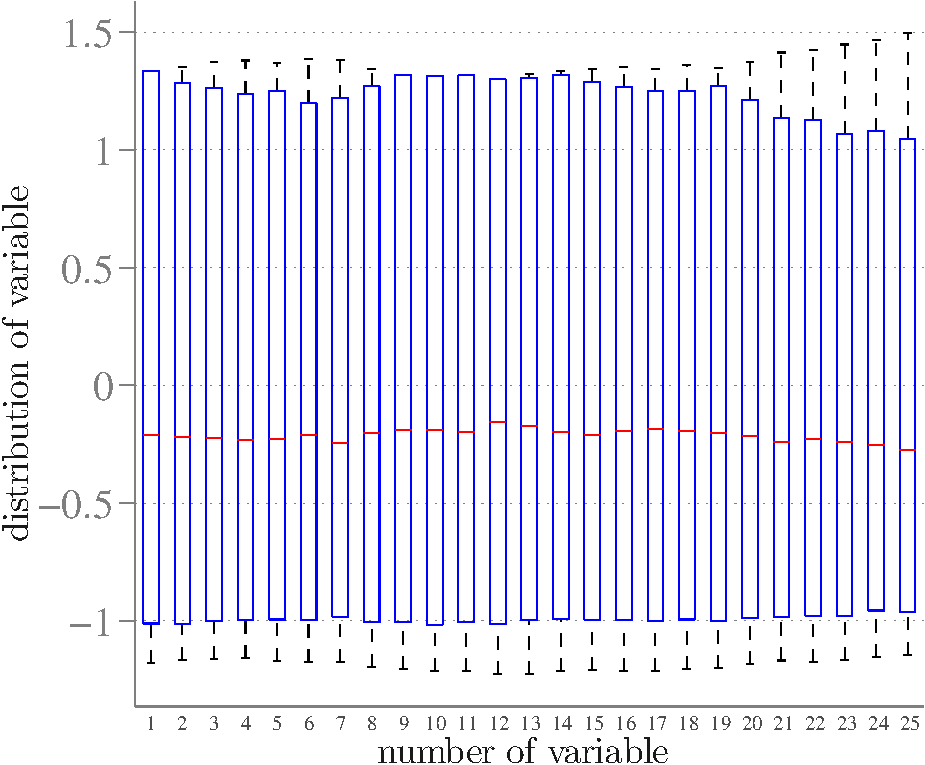
\includegraphics[height=1.8in]{../figures/boxplot2-crop.pdf} \label{fig:boxplot2}}
  \caption{Box plots of part of the data before \ref{fig:boxplot1} and after \ref{fig:boxplot2} normalization. Rest of the data looks similar.}
\end{figure}
  
  Since there are $9360$ numbers for one picture using all of them will lead to ill-conditioning (there is more features than pictures). We calculated correlation of them with output and we obtained picture of an abstract person, see \ref{fig:correlation}.
  Also on figure \ref{fig:correlations} we can see that there are regions and gradients more and less important for this task and they have shape of a person. Values of correlation were between $-0.37$ and $0.37$
  \begin{figure}[t]
    \center
    \subfigure[Absolute value of correlation for different directions of gradient]{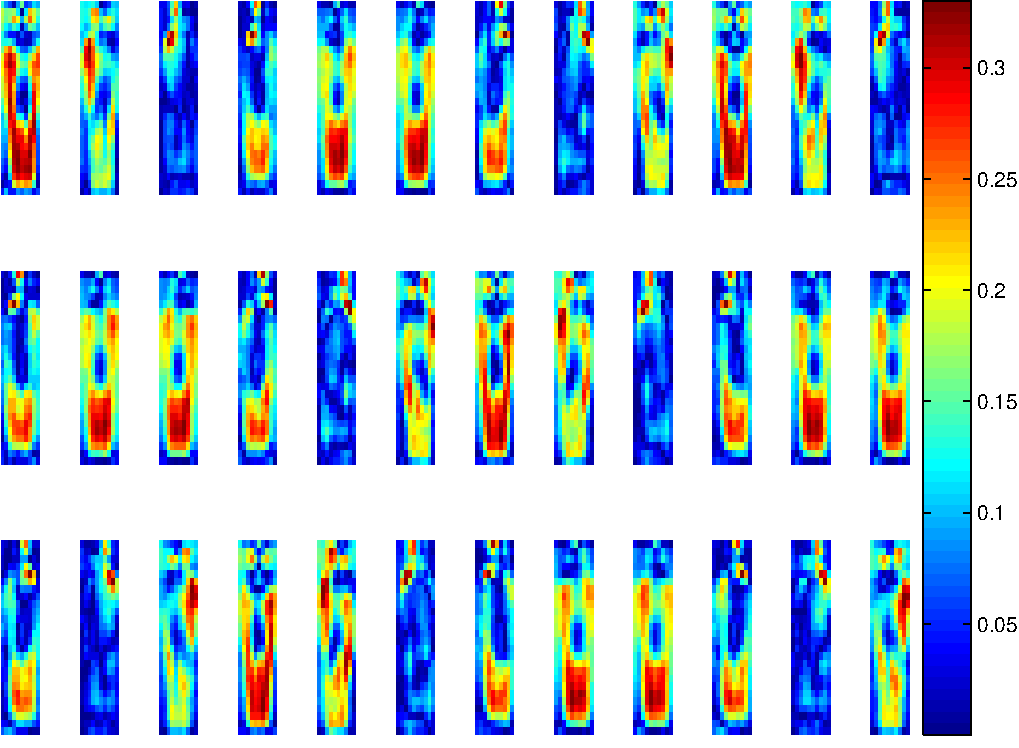
\includegraphics[height=1.7in]{../figures/absoluteCorelation-crop.pdf} \label{fig:correlations}}
      \;\;\;
    \subfigure[positive correlation]{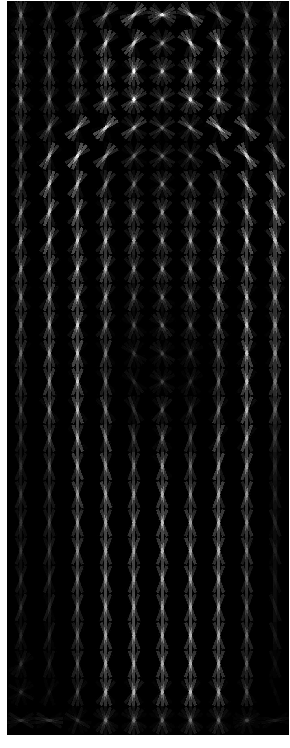
\includegraphics[height=1.7in]		{../figures/averagePerson-crop.pdf} \label{fig:correlation}}
    \caption{Absolute value \ref{fig:correlations} and only positive part \ref{fig:correlation} of correlation, plotted as a feature. There is a lot of not correlated data (deep blue).}
  \end{figure}
  To overcome the problem of huge number of features, we thought about removing those with little correlation to labels. This (empirically) did not work well, so we moved to other methods. One of them is singular value decomposition (i.e. taking only some vectors corresponding to the biggest singular values). This proved to be a better idea, because correlation captures only linear dependence and don't capture structure in the data. We have done SVD (i.e. we used MatLab's \verb+svds+ function) for $1000$ singular values and then used $8545\times1000$ as our new train matrix for testing different methods.
  
 We planned to do SVD again for bigger number of singular values later, if we would need it. But every method we tried was performing better for even smaller subsets of those $1000$ features (ex. $200$, corresponding to $200$ biggest singular values), in all cases due to high variance. To choose a good subset of features (after SVD), we used F-score feature selection (explained e.g. in \cite{fscore}) from libsvm library tools \cite{fselection}.
  This method estimates how much of particular variable variance  is correlated to output. We used it after SVD for two reasons: first - F-score, the same as correlation, don't take into account higher structure of the data and second - running F-score feature selection on all features required to much time and memory.

% TODO: test matrices descriptions.

\section{Applied methods}
We tried to apply many methods for this task, for most of them we used existing libraries. To check which method is better we were doing $5$-fold cross-validation and then plotted ROC for both test and train predictions. That was giving us an estimate how good performance is of particular method.

\subsection{Penalized logistic regression}
We started with the the simple (penalized) logistic regression. Not surprisingly, this method had quite big bias. What's interesting, when we were using $1000$ features (from SVD) it also had a big variance. Setting bigger penalty ($\lambda$) caused even bigger bias and very poor performance. Decreasing number of features helped decreasing variance. Penalized logistic regression was working the best with only about $120$ features with biggest singular values in SVD and $\lambda = 0.1$, and gave average TPR $0.831$ (see \ref{fig:ROClinear})

% We tried to use the most correlated part of all of the data (without decomposition), but to then penalized logistic regression needed more data (and more time) and was performing much poorer. At that point we abandoned using not decomposed data, because we expected that using the most correlated data should be the best suited for simple model like penalized logistic regression.

Then we used data selected by F-score and it improved slightly. We used the same number of variables $120$ and the same $\lambda = 0.1$, which seemed to be the best also in this case. Average TPR was $0.865$, as shown in the figure: \ref{fig:ROClinear2}.
% [p1,p2,y] = crossValidation(labels(permutacja),U(permutacja,1:120),4,0.1);
  \begin{figure}[h]
    \center
    \subfigure[ROC curves for penalized logistic regression (test and train data) compared with random assignment.]{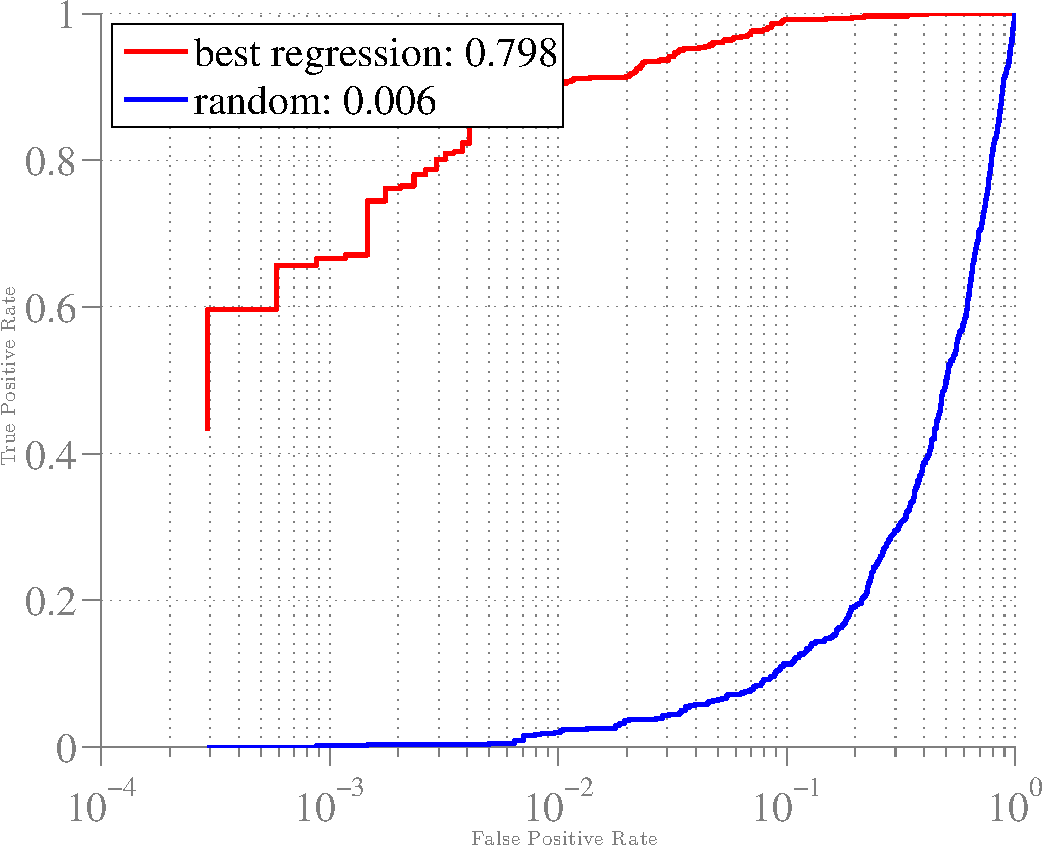
\includegraphics[height=1.7in]{../figures/ROClinear-crop.pdf} \label{fig:ROClinear}}
    \subfigure[ROC curves for penalized logistic regression (test and train data) when using data with the best F-score]{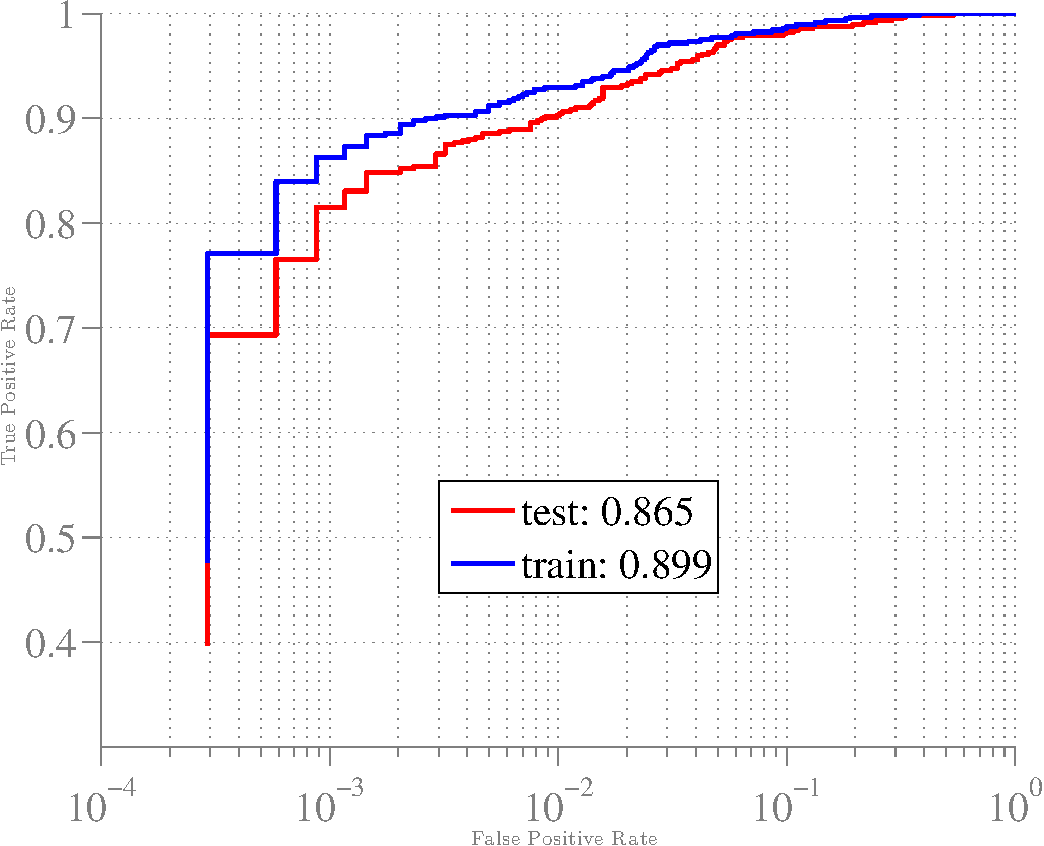
\includegraphics[height=1.7in]{../figures/ROClinear2-crop.pdf} \label{fig:ROClinear2}}
    \caption{ROC curves for two best logistic regression models. \ref{fig:ROClinear2} has better average TPR, but \ref{fig:ROClinear} performs better for small False Positive Rate, what crucial in this task.}
  \end{figure}

\subsection{Support Vector Machine}
For SVM we used LIBSVM library \cite{libsvm}.
We tried different kernels for SVM, but didn't try to construct  one. We used libsvm built-in tool (\texttt{grid.py}) to grid search for parameters of kernel, and then tried to tune them by hand, but it didn't give much improvement. More significant was changing amount of features in the models. We think optimal value was about $120$. For all SVM models we obtained similar TPR, about $0.85$, but they didn't do well with small values of False Positive Rate.

  \begin{figure}[h]
    \center
    \subfigure[ROC curves for SVMs, rbf-kernel and linear-kernel.]{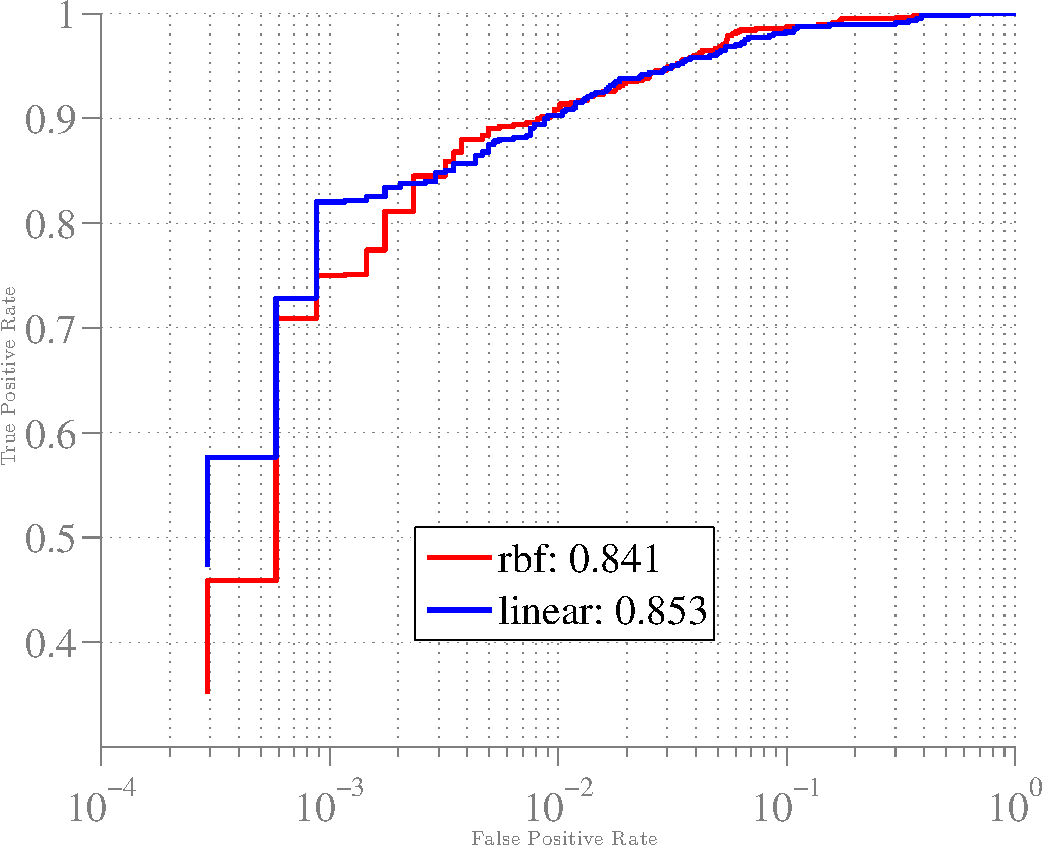
\includegraphics[height=1.7in]{../figures/ROCSVM-crop.pdf} \label{fig:ROCSVM}}
    \subfigure[ROC curves for test and train of SVM with RBF kernel. It looks like overfitting.]{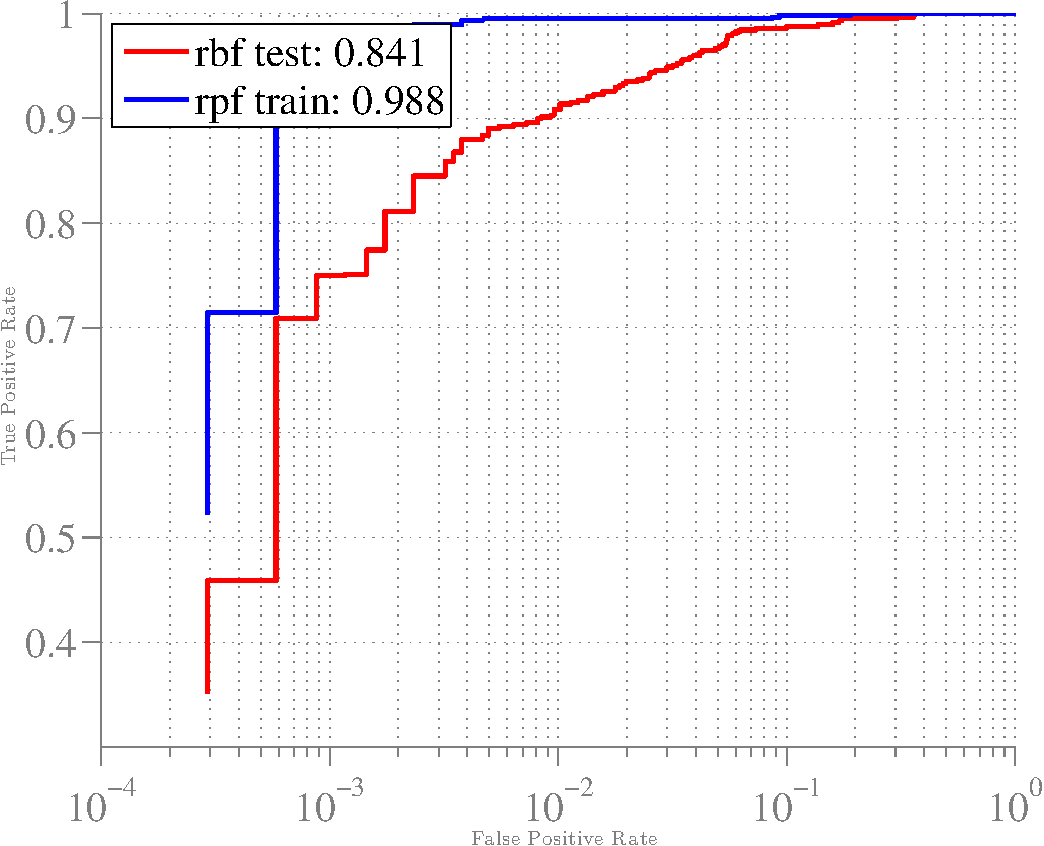
\includegraphics[height=1.7in]{../figures/ROCSVMtrain-crop.pdf} \label{fig:ROCSVM}}
    \caption{ROC curves for SVMs.}
  \end{figure}

\subsection{Neural Networks}
For Neural Network we used deep learning toolbox \cite{deep}. We tuned the parameters and obtained the best performance for $2$ layers, first of $50$ hidden variables and second of $2$ hidden variables and sigmoid activation function (\ref{fig:ROCneural}). To train it, we used all the data. We tried to run it on decomposed matrix too, but it was working half that good. It's not surprising, since Neural Network is supposed to capture abstraction from data and SVD (with taking only some features) may destroyed some structure. But even for Neural Network using $200$ features after SVD was performing better than using $1000$ of them.

  \begin{figure}[h]
    \center
    \subfigure[ROC curves for best tuned Neural Network and random choice.]{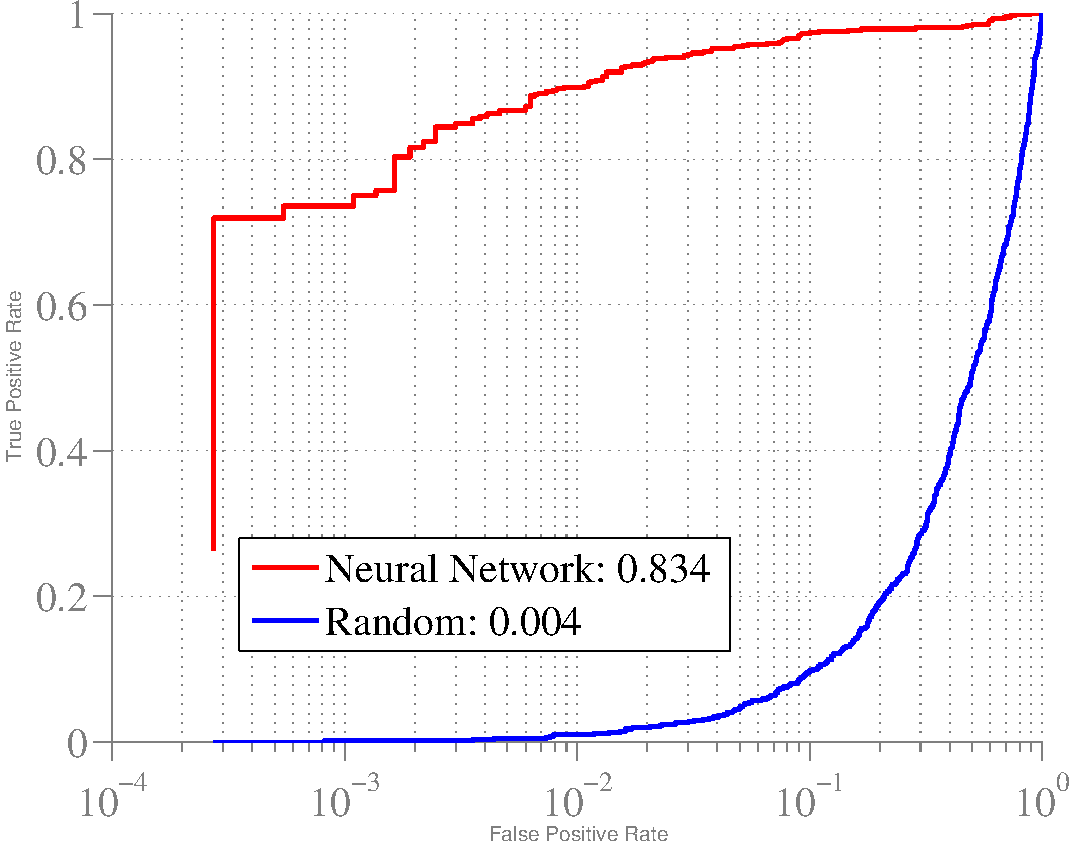
\includegraphics[height=1.7in]{../figures/ROCneural-crop.pdf} \label{fig:ROCneural}}
     \subfigure[ROC curves for test and train for Random Forest for 2000 trees and 100 variables. It looks like random forest is overfitting.]{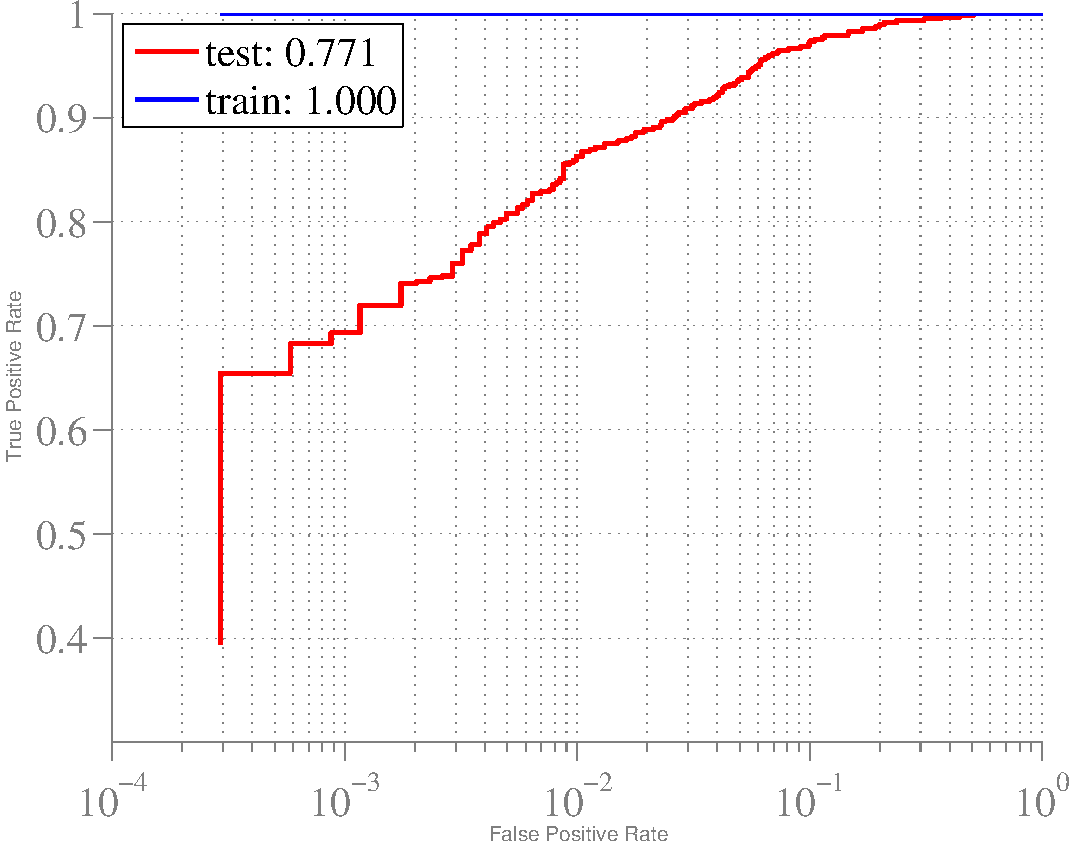
\includegraphics[height=1.7in]{../figures/ROCtree-crop.pdf} \label{fig:ROCtree}}
    \caption{ROC curves for Neural Network \ref{fig:ROCneural} and Random Forest \ref{fig:ROCtree}}
  \end{figure}

\subsection{Random Forest}

For Random Forest we used randomforest-matlab library\cite{rf}.
We were taking predictions for single trees and averaging them, and treated this average as probability of point belonging to specific class.
When we were using default number of trees and number of variables sampled in each split (\verb+mtry+), Random Forest suffered from big variance. We tried to fix it by increasing number of trees, but it didn't help much.
We tried also to change \verb+mtry+, but it seemed that default (square root of number of variables) works best. 

To sum up, Random Forest performed poorer than other methods.
We think that it may be good idea to try using this method not for predictions, but for choosing most important features, but we didn't managed to do this.

\end{document}
